\section{Sugestões \& Recomendações}

\subsection{Acidentes em Braga no ano de 2019}

Ao longo do desenvolvimento do nosso projeto percebemos, analisando os resultados finais, que existe uma diferença muito pouco definida entre o conjunto de classes $\{\mbox{\texttt{Low}, \texttt{Medium}, \texttt{High}}\}$ pelo que o nosso modelo, segundo as curvas ROC, é péssimo a distinguir entre estas classes. Apesar de ser muito bom a distinguir entre as classes $\{\mbox{\texttt{None}, \texttt{Very High}}\}$, uma performance na melhoria da accuracy está diretamente relacionada com a boa separação classes, o que não é de todo garantido com o modelo atual. 

\begin{figure}[H]
    \centering
    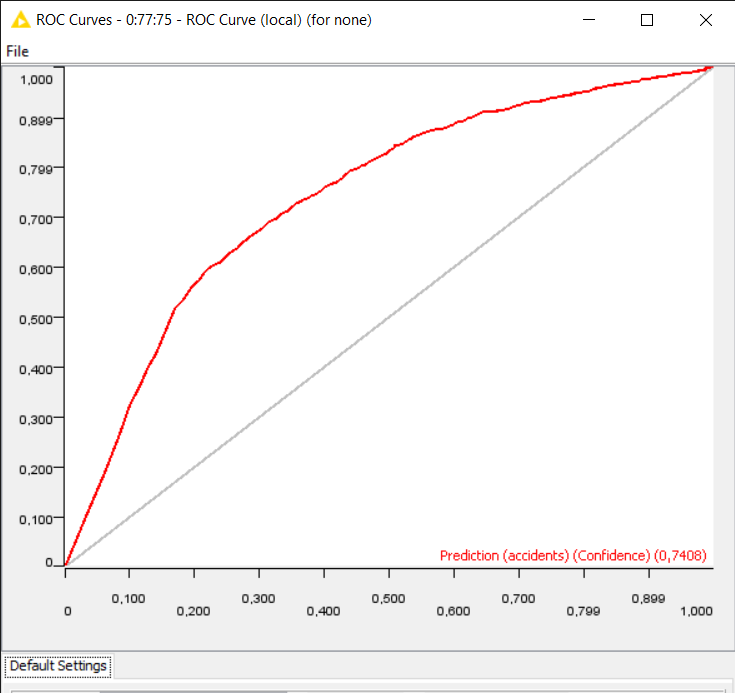
\includegraphics[width=0.4\linewidth]{Figures/ROC/none.png}
    \caption{Curva de ROC para a classe \texttt{None}.}
    \label{fig:ii1}
\end{figure}

\begin{figure}[H]
    \centering
    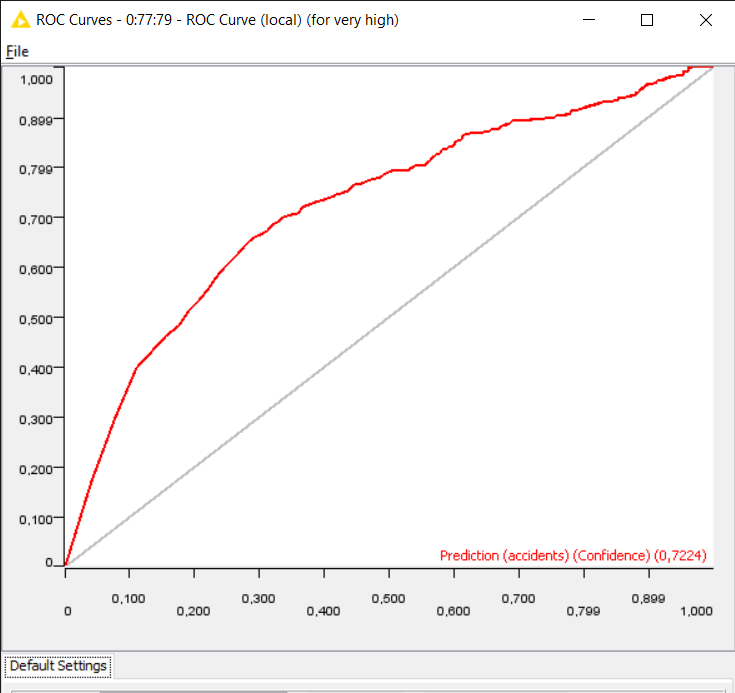
\includegraphics[width=0.4\linewidth]{Figures/ROC/very high.png}
    \caption{Curva de ROC para a classe \texttt{Very High}.}
    \label{fig:ii2}
\end{figure}

Como podemos ver pelas figuras \ref{fig:ii1} e \ref{fig:ii2} rapidamente percebemos que o nosso modelo consegue fazer uma boa distinção entre estas duas. No entanto, se olharmos para as figuras \ref{fig:ii3}, \ref{fig:ii4} e \ref{fig:ii5}, rapidamente percebemos que o nosso modelo é péssimo nestas classes.

\begin{figure}[H]
    \centering
    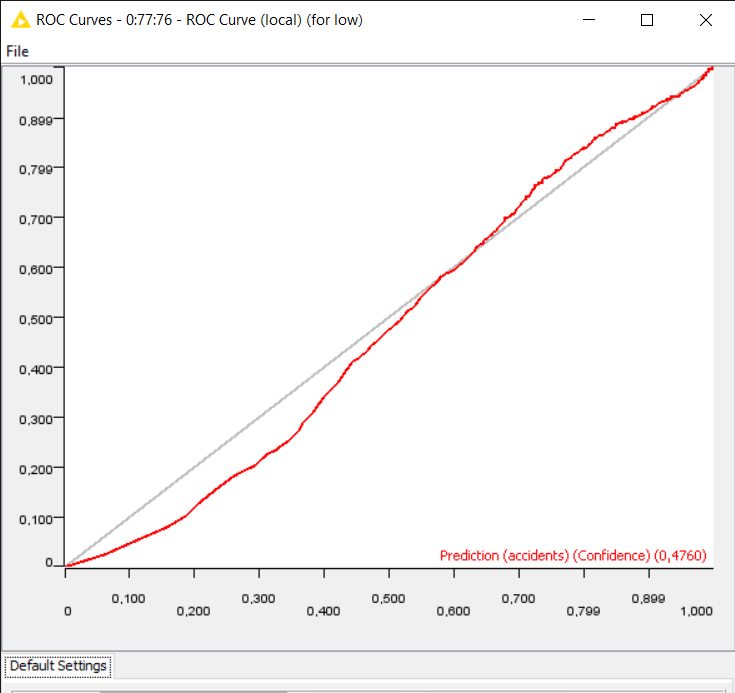
\includegraphics[width=0.4\linewidth]{Figures/ROC/low.png}
    \caption{Curva de ROC para a classe \texttt{Low}.}
    \label{fig:ii3}
\end{figure}

\begin{figure}[H]
    \centering
    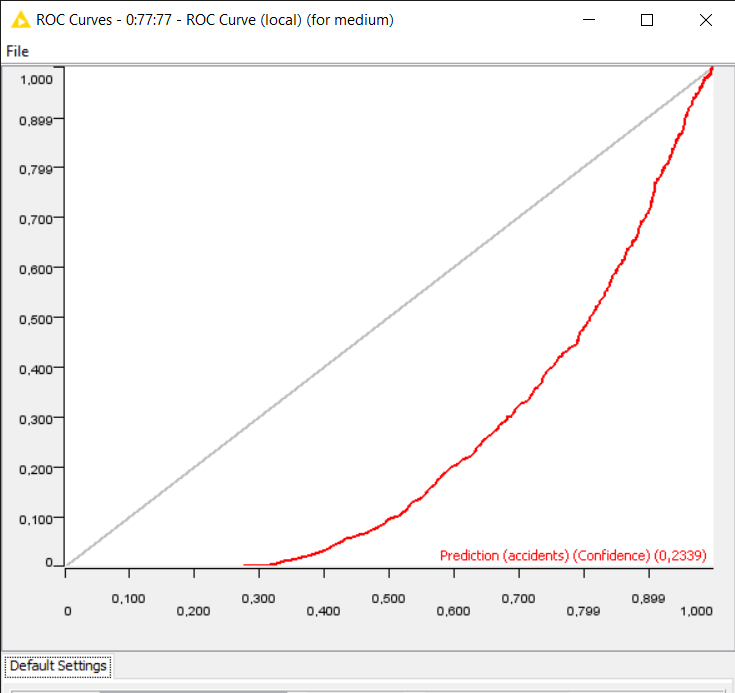
\includegraphics[width=0.4\linewidth]{Figures/ROC/medium.png}
    \caption{Curva de ROC para a classe \texttt{Medium}.}
    \label{fig:ii4}
\end{figure}

\begin{figure}[H]
    \centering
    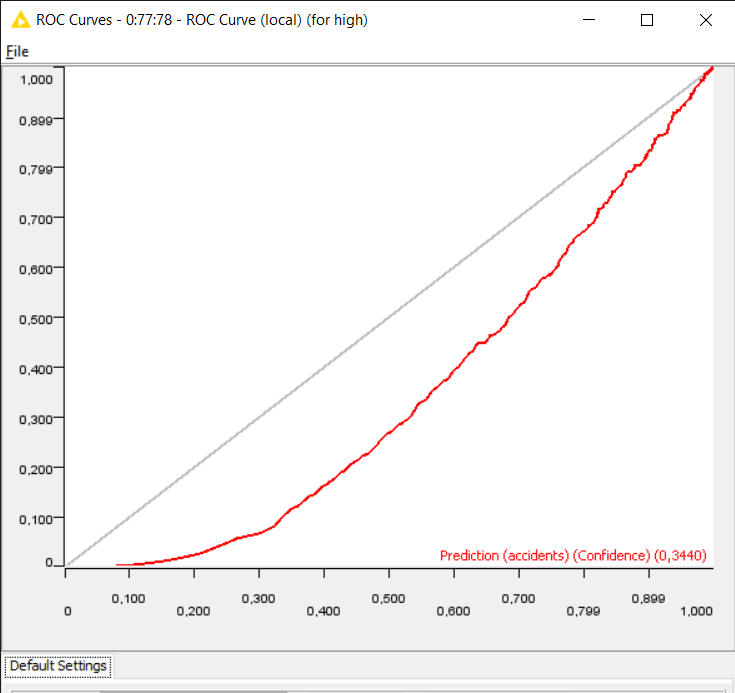
\includegraphics[width=0.4\linewidth]{Figures/ROC/high.png}
    \caption{Curva de ROC para a classe \texttt{High}.}
    \label{fig:ii5}
\end{figure}

\subsection{League of Legends}

Apesar dos resultados bastante promissores apenas com os primeiros 10 minutos de jogo, é notável que, num jogo com dinâmicas tão complexas, utilizar apenas os primeiros 10 minutos é pouco representativo no resultado final.

Existem muitos objetivos, como batalhas em equipa e obtenção de monstros épicos que fornecem pontos de viragem cruciais em jogos, que tendem a concentrarem-se em períodos após os primeiros 10 minutos.

Como tal, e em formato de recomendação, ponderamos que com um aumento do número de minutos considerados poderemos vir a obter \textit{accuracies} mais elavadas.